\documentclass[tikz,border=10pt]{standalone}
\usepackage{tikz}
\usetikzlibrary{shapes, arrows, positioning, calc, fit}

\begin{document}

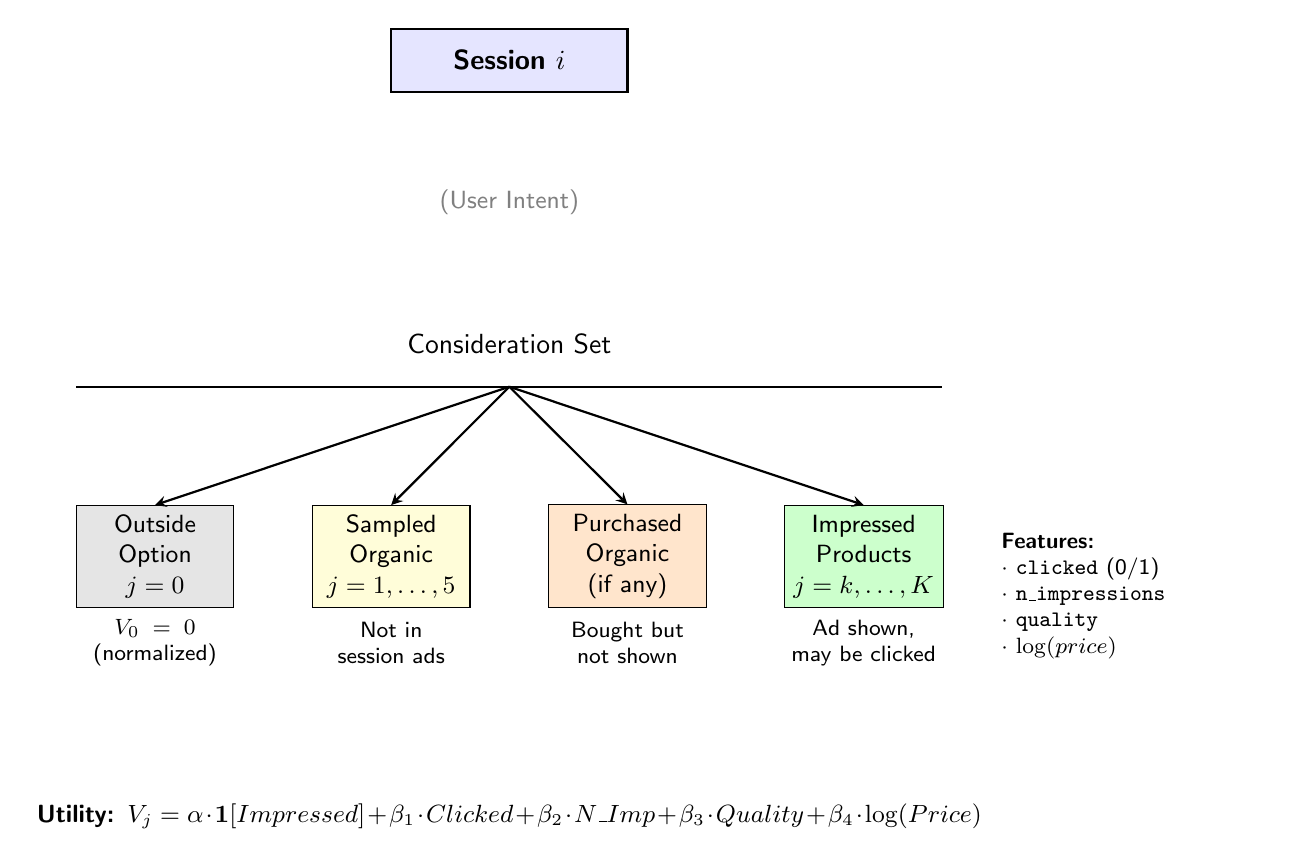
\begin{tikzpicture}[node distance=1.5cm, auto, >=stealth]

    % Session node at top
    \node (session) [rectangle, draw, thick, fill=blue!10, minimum width=3cm, minimum height=0.8cm, font=\sffamily\bfseries] {Session $i$};

    \node (intent) [below of=session, yshift=-0.3cm, font=\sffamily\small, text=gray] {(User Intent)};

    % Consideration set label
    \node (cset) [below of=intent, yshift=-0.3cm, font=\sffamily] {Consideration Set};

    % Horizontal line
    \draw[thick] ($(cset.south) + (-5.5cm,-0.3cm)$) -- ($(cset.south) + (5.5cm,-0.3cm)$);

    % Alternative nodes
    \node (outside) [rectangle, draw, below of=cset, xshift=-4.5cm, yshift=-1.2cm,
                     minimum width=2cm, minimum height=1.2cm, font=\sffamily\small, align=center,
                     fill=gray!20] {Outside\\Option\\$j=0$};

    \node (sampled) [rectangle, draw, below of=cset, xshift=-1.5cm, yshift=-1.2cm,
                     minimum width=2cm, minimum height=1.2cm, font=\sffamily\small, align=center,
                     fill=yellow!15] {Sampled\\Organic\\$j=1,\ldots,5$};

    \node (purchased) [rectangle, draw, below of=cset, xshift=1.5cm, yshift=-1.2cm,
                       minimum width=2cm, minimum height=1.2cm, font=\sffamily\small, align=center,
                       fill=orange!20] {Purchased\\Organic\\(if any)};

    \node (impressed) [rectangle, draw, below of=cset, xshift=4.5cm, yshift=-1.2cm,
                       minimum width=2cm, minimum height=1.2cm, font=\sffamily\small, align=center,
                       fill=green!20] {Impressed\\Products\\$j=k,\ldots,K$};

    % Arrows from session to alternatives
    \draw[->, thick] ($(cset.south) + (0,-0.3cm)$) -- (outside.north);
    \draw[->, thick] ($(cset.south) + (0,-0.3cm)$) -- (sampled.north);
    \draw[->, thick] ($(cset.south) + (0,-0.3cm)$) -- (purchased.north);
    \draw[->, thick] ($(cset.south) + (0,-0.3cm)$) -- (impressed.north);

    % Labels below alternatives
    \node[below of=outside, yshift=0.4cm, font=\footnotesize\sffamily, text width=2.2cm, align=center] {$V_0 = 0$\\(normalized)};

    \node[below of=sampled, yshift=0.4cm, font=\footnotesize\sffamily, text width=2.2cm, align=center] {Not in\\session ads};

    \node[below of=purchased, yshift=0.4cm, font=\footnotesize\sffamily, text width=2.2cm, align=center] {Bought but\\not shown};

    \node[below of=impressed, yshift=0.4cm, font=\footnotesize\sffamily, text width=2.2cm, align=center] {Ad shown,\\may be clicked};

    % Feature box for impressed products
    \node[right of=impressed, xshift=2cm, yshift=-0.5cm, font=\footnotesize\sffamily,
          text width=3.5cm, align=left] {
        \textbf{Features:}\\
        $\cdot$ \texttt{clicked} (0/1)\\
        $\cdot$ \texttt{n\_impressions}\\
        $\cdot$ \texttt{quality}\\
        $\cdot$ $\log(\text{price})$
    };

    % Utility equation
    \node[below of=cset, yshift=-4.5cm, font=\sffamily\small, text width=12cm, align=center] {
        \textbf{Utility:} $V_j = \alpha \cdot \mathbf{1}[\text{Impressed}] + \beta_1 \cdot \text{Clicked} + \beta_2 \cdot \text{N\_Imp} + \beta_3 \cdot \text{Quality} + \beta_4 \cdot \log(\text{Price})$
    };

\end{tikzpicture}

\end{document}
